\section{Results}
\label{sec:results}

We present results by hypothesis: classification spread (\secref{sec:res_cls}), length (\secref{sec:res_len}), compliance (\secref{sec:res_caps}), extraction (\secref{sec:res_ext}), and scale (\secref{sec:res_scale}). We close with the noise floor and the consistency of edit effects across models (\secref{sec:res_noise}).

%---------------------------------------------------------------
\subsection{Surface Edits Shift Classification Accuracy, Mostly in Small Models (H1)}
\label{sec:res_cls}

\begin{figure}[t]
    \centering
    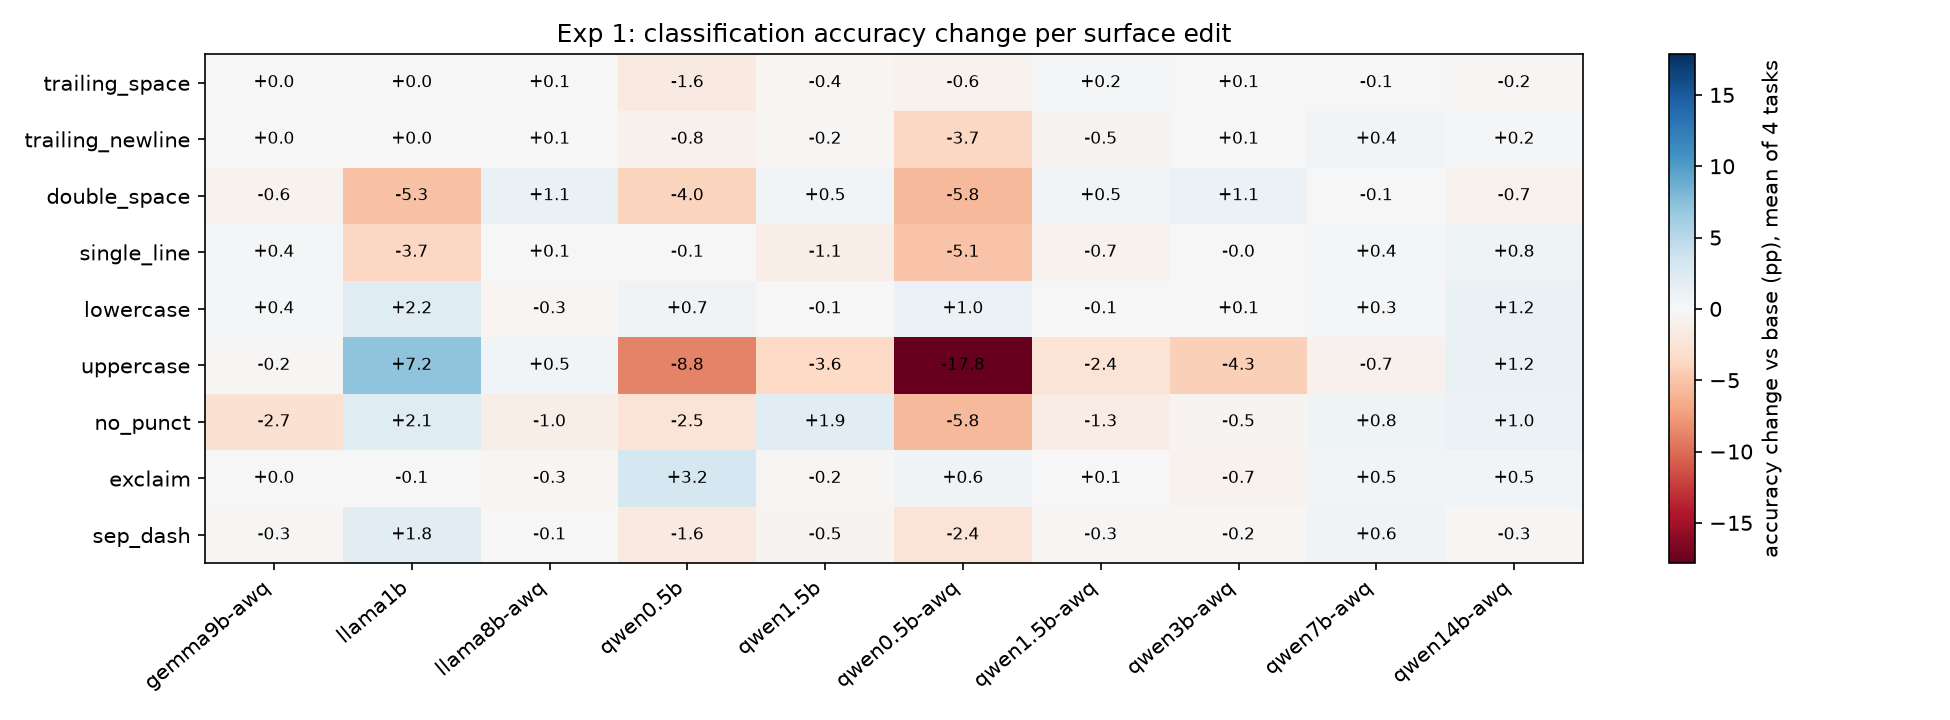
\includegraphics[width=0.95\linewidth]{figures/cls_delta_heatmap.png}
    \caption{Classification accuracy change (pp) of each surface edit relative to \edit{base}, averaged over \sst, \agnews, \emotion, and \boolq. Red cells mark accuracy losses and blue cells mark gains. ALL-CAPS (\capsedit) causes the largest losses in small \qwen models (up to $-17.8$ on average for qwen0.5b-awq) but \emph{raises} accuracy for llama1b ($+7.2$). Trailing whitespace is a byte-identical placebo for \llama and \gemma (exactly 0.0 or 0.1) and has small effects elsewhere. Models of 7B parameters or more have $|\Delta|\leq 1.2$ for every edit except \edit{no\_punct} on \gemma-9B ($-2.7$).}
    \label{fig:heatmap}
\end{figure}

\begin{table}[t]
    \centering
    \small
    \caption{Accuracy spread (max $-$ min over 10 variants, pp) per model and task. Parentheses: mean spread under the permutation null (no format effect). $^*$: spread exceeds the null at $p<0.05$. Lowest spread per column in \textbf{bold}. Models are sorted by size. Models of 1.2B parameters or fewer show 7--28 pp spreads. At 7--14B, only \agnews consistently exceeds the null by a wide margin.}
    \label{tab:spread}
    \begin{tabular}{@{}lccccc@{}}
        \toprule
        \textbf{Model} & \sst & \agnews & \emotion & \boolq & \textbf{Mean} \\
        \midrule
        qwen0.5b      & 11.0 (2.2)$^*$ & 24.0 (4.0)$^*$ & 14.4 (4.1)$^*$ & 6.7 (4.3)$^*$ & 14.0 \\
        qwen0.5b-awq  & 28.0 (3.6)$^*$ & 22.4 (4.4)$^*$ & 26.4 (4.4)$^*$ & 8.3 (5.3)$^*$ & 21.3 \\
        llama1b       & 14.8 (2.7)$^*$ & 20.0 (3.1)$^*$ & 7.2 (3.6)$^*$ & 25.7 (5.4)$^*$ & 16.9 \\
        qwen1.5b      & 2.2 (1.3)$^*$ & 20.4 (3.2)$^*$ & 2.4 (2.9) & 2.3 (2.8) & 6.8 \\
        qwen1.5b-awq  & 1.2 (1.3) & 11.2 (2.8)$^*$ & 6.0 (3.1)$^*$ & 3.3 (3.0) & 5.4 \\
        qwen3b-awq    & 3.8 (1.5)$^*$ & 10.6 (2.4)$^*$ & 8.8 (2.9)$^*$ & \textbf{1.3} (2.3) & 6.1 \\
        qwen7b-awq    & 1.8 (1.2) & 9.8 (2.3)$^*$ & \textbf{2.0} (2.1) & 2.0 (1.7) & \textbf{3.9} \\
        llama8b-awq   & \textbf{1.0} (1.3) & 10.6 (3.1)$^*$ & 4.2 (2.5)$^*$ & 2.7 (2.3) & 4.6 \\
        gemma9b-awq   & \textbf{1.0} (0.7) & 14.2 (2.4)$^*$ & 2.8 (2.0) & 1.7 (1.3) & 4.9 \\
        qwen14b-awq   & 2.6 (1.2)$^*$ & \textbf{3.8} (2.0)$^*$ & 5.6 (2.5)$^*$ & 3.7 (2.4)$^*$ & \textbf{3.9} \\
        \bottomrule
    \end{tabular}
\end{table}

\Figref{fig:heatmap} shows the mean accuracy change of each edit, and \tabref{tab:spread} shows the resulting spread per model and task.

\para{Format effects are real and often large.} Over the 40 model$\times$task cells, the median spread is 5.8 points (IQR 2.4--11.9; range 1.0--28.0). The spread exceeds the permutation null in 27 of 40 cells. Of the 360 variant-vs-base tests, 48 are significant after Holm correction. The edits do not contribute equally: \capsedit accounts for 16 of the 48 significant changes, followed by \edit{no\_punct} (9), \edit{single\_line} (6), \edit{double\_space}, \lowedit, and \edit{trailing\_newline} (4 each), \edit{exclaim} and \edit{sep\_dash} (2 each), and \edit{trailing\_space} (1). The mean prediction flip rate relative to \edit{base} follows the same order: 17.6\% for \capsedit, 14.7\% for \edit{no\_punct}, 9.8\% for \edit{double\_space}, and only 1.6\% for \edit{trailing\_space}.

\para{ALL-CAPS hurts small models only.} The largest single effect is $-27$ points for qwen0.5b-awq on \sst. Averaged over tasks, \capsedit costs $-17.8$ (qwen0.5b-awq), $-8.8$ (qwen0.5b), and $-2.4$ to $-4.3$ points (\qwen 1.5B--3B). For models of 7B or more the effect is near zero ($-0.7$ to $+1.2$). The sign is not universal: llama1b \emph{gains} 7.2 points under ALL-CAPS.

\para{\agnews drives most of the large-model spread.} \agnews is the most format-sensitive task, with spread $\geq$9.8 points for every model except qwen14b-awq. Inspecting the outputs, most of this swing comes from \emph{label-vocabulary drift}: under some formats, models answer with labels outside the allowed list, such as ``politics'' for \emph{world} or ``news'', and how often they do so depends on the format. For models of 7B or more, spreads on \sst, \emotion, and \boolq lie within about 2 points of the permutation null.

\para{Verdict on H1: partially supported.} Format-induced differences are real and usually significant. The 3--8 point range describes the 1.5B--14B models on average (3.9--6.8 points). Models of 1.2B or fewer reach 14--21 points on average, well above the hypothesized range, and at 7--14B much of the remaining spread outside \agnews is at noise level.

%---------------------------------------------------------------
\subsection{Trailing Whitespace Does Not Lengthen Outputs (H2)}
\label{sec:res_len}

\begin{table}[t]
    \centering
    \small
    \caption{\ifeval results. \emph{Left}: ratio of mean response length (tokens) under each variant to \edit{base}, with 95\% bootstrap CI for trailing whitespace. $^\dagger$: placebo, since the chat template trims trailing whitespace. $^*$: Wilcoxon $p<0.05$. \emph{Right}: prompt-level strict accuracy at \edit{base} and change (pp) under ALL-CAPS (with 95\% CI) and lowercase. ``excl.'' removes prompts with letter-case instructions. \textbf{Bold}: McNemar $p<0.05$ (uncorrected). All nine ALL-CAPS estimates are negative.}
    \label{tab:ifeval}
    \resizebox{\textwidth}{!}{%
    \begin{tabular}{@{}lcccccccc@{}}
        \toprule
        & \multicolumn{4}{c}{\textbf{Length ratio (variant / base)}} & \multicolumn{4}{c}{\textbf{Strict compliance (pp)}} \\
        \cmidrule(lr){2-5} \cmidrule(lr){6-9}
        \textbf{Model} & \edit{trailing\_space} & \edit{trailing\_newline} & \edit{trailing\_2newline} & \capsedit & \edit{base} & \capsedit $\Delta$ & \lowedit $\Delta$ & \capsedit $\Delta$ excl. \\
        \midrule
        qwen0.5b      & 0.95 [0.90, 1.00] & 0.94 [0.88, 1.00] & 0.95 [0.89, 1.01] & 1.03 & 27.2 & \textbf{$-$5.7} [$-$9.8, $-$1.8] & $-$3.9 & $-$7.2 \\
        qwen0.5b-awq  & 1.00 [0.95, 1.04] & 0.95 [0.90, 1.02] & 0.99 [0.93, 1.05] & 1.00 & 27.4 & \textbf{$-$6.7} [$-$10.7, $-$2.6] & $-$4.3 & $-$8.3 \\
        llama1b$^\dagger$ & 0.99 [0.96, 1.03] & 0.99 [0.96, 1.03] & 0.98 [0.95, 1.02] & 1.05$^*$ & 47.9 & \textbf{$-$4.4} [$-$8.1, $-$0.4] & $-$0.7 & $-$5.9 \\
        qwen1.5b      & 1.02 [0.96, 1.08] & 0.98 [0.92, 1.04] & 1.07 [1.01, 1.14] & 1.10$^*$ & 41.4 & $-$3.9 [$-$7.9, $-$0.2] & $-$3.3 & $-$5.9 \\
        qwen1.5b-awq  & 0.96 [0.91, 1.00] & 0.97 [0.91, 1.03] & 0.99 [0.93, 1.06] & 1.01 & 37.5 & $-$3.7 [$-$7.4, 0.2] & $-$3.3 & $-$4.4 \\
        qwen3b-awq    & 0.98 [0.93, 1.04] & 1.02 [0.96, 1.09] & 0.98 [0.92, 1.05] & 1.01$^*$ & 58.2 & $-$3.3 [$-$7.6, 0.9] & $-$3.5 & $-$4.6 \\
        qwen7b-awq    & 1.00 [0.97, 1.02] & 1.01 [0.97, 1.05] & 1.02 [0.98, 1.06] & 1.05$^*$ & 71.7 & \textbf{$-$4.4} [$-$8.1, $-$0.9] & $-$2.8 & $-$4.2 \\
        llama8b-awq$^\dagger$ & 1.00 [1.00, 1.01] & 1.00 [1.00, 1.01] & 0.99 [0.98, 1.00] & 1.03$^*$ & 74.1 & $-$3.1 [$-$6.7, 0.6] & $-$2.2 & $-$2.6 \\
        qwen14b-awq   & 0.98 [0.95, 1.00] & 0.99 [0.96, 1.03] & 1.00 [0.96, 1.03] & 1.02$^*$ & 77.8 & \textbf{$-$3.7} [$-$7.2, $-$0.4] & $-$2.0 & $-$5.0 \\
        \bottomrule
    \end{tabular}
    }
\end{table}

The left half of \tabref{tab:ifeval} reports length ratios on \ifeval. Trailing-whitespace ratios lie between 0.94 and 1.07 and fall on both sides of 1. None of the 21 \qwen trailing-whitespace comparisons is significant (smallest Wilcoxon $p=0.06$). This variation matches the placebo models (0.98--1.00) and the replicate run (0.985), so it is consistent with noise. For \llama and \gemma the edit cannot have any effect, because their chat templates strip trailing whitespace. In contrast, ALL-CAPS prompts make answers slightly \emph{longer} ($+1$ to $+10\%$, significant for 6 of 9 models).

\para{Verdict on H2: refuted.} The largest point estimate is $+7\%$, well short of the hypothesized 15--25\%, and no trailing-whitespace effect is significant. A plausible source of the belief is raw completion-mode prompting, where a trailing space changes tokenization at the point where generation starts. In a chat template the whitespace comes before the end-of-turn token, and two of the three families remove it.

%---------------------------------------------------------------
\subsection{ALL-CAPS Lowers Instruction Compliance at Every Size (H3)}
\label{sec:res_caps}

\begin{figure}[t]
    \centering
    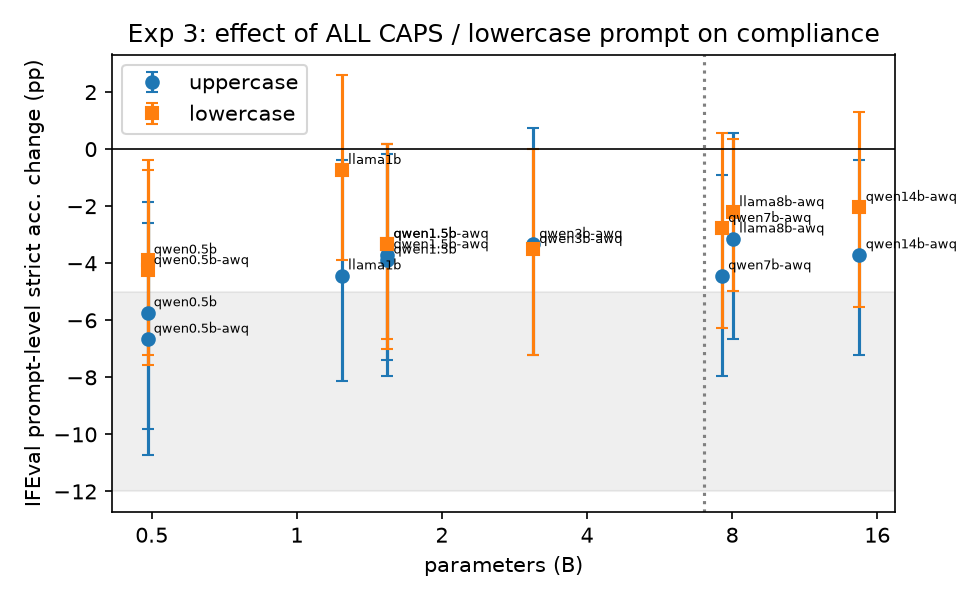
\includegraphics[width=0.62\linewidth]{figures/caps_compliance.png}
    \caption{Change in \ifeval prompt-level strict accuracy under ALL-CAPS (blue) and lowercase (orange) prompts, with 95\% bootstrap CIs. The shaded band is the hypothesized 5--12 pp drop for small models, and the dotted line marks 7B. All ALL-CAPS estimates are negative, including at 7--14B, where H3 predicted no effect. Lowercase also hurts, so the cause is non-canonical casing rather than ``shouting''.}
    \label{fig:caps}
\end{figure}

The right half of \tabref{tab:ifeval} and \figref{fig:caps} show the compliance results. All nine ALL-CAPS point estimates are negative, and five are significant: both 0.5B models, llama1b, qwen7b-awq ($-4.4$, $p=0.02$), and qwen14b-awq ($-3.7$, $p=0.04$). Excluding prompts whose instructions concern letter case leaves the effects similar or larger ($-2.6$ to $-8.3$), so the drop is not an artifact of case-related instructions. Lowercasing also lowers compliance ($-0.7$ to $-4.3$), though less than upper-casing. This suggests that the harm comes from non-canonical casing in general rather than from ``shouting'' specifically. The effect shrinks only slightly with scale: $+1.6$ points per tenfold increase in parameters ($p=0.028$, $\rho=0.79$ across nine models; not significant within the 5-model \qwen-AWQ ladder, $p=0.23$).

\para{Verdict on H3: partially supported.} Only the 0.5B models fall in the predicted 5--12 point range. At 7--14B the effect is $-3.1$ to $-4.4$ points, which is not negligible: it is significant for two of three models, although it sits close to the 1--3 point inference noise floor (\secref{sec:res_noise}).

%---------------------------------------------------------------
\subsection{JSON Prompts Do Not Uniformly Improve Extraction (H4)}
\label{sec:res_ext}

\begin{table}[t]
    \centering
    \small
    \caption{Extraction F1 ($\times$100). ``Plain'': F1 with plain input and plain output. ``JSON in'': main effect of wrapping the input in JSON, averaged over output formats, with 95\% paired bootstrap CI. ``JSON out'': effect of requesting JSON output with plain input. \textbf{Bold}: CI excludes zero and the effect is positive. Requested JSON was valid in 86--100\% of responses. No model gains 10--15 points on both tasks.}
    \label{tab:extraction}
    \resizebox{\textwidth}{!}{%
    \begin{tabular}{@{}lcccccc@{}}
        \toprule
        & \multicolumn{3}{c}{\squad (span QA)} & \multicolumn{3}{c}{\conll (NER)} \\
        \cmidrule(lr){2-4} \cmidrule(lr){5-7}
        \textbf{Model} & Plain & JSON in $\Delta$ & JSON out $\Delta$ & Plain & JSON in $\Delta$ & JSON out $\Delta$ \\
        \midrule
        qwen0.5b      & 59.7 & $-$4.4 [$-$6.7, $-$2.1] & $+$11.2 & 17.1 & $-$5.5 [$-$7.4, $-$3.7] & $-$1.1 \\
        qwen0.5b-awq  & 49.9 & $-$13.5 [$-$16.5, $-$10.4] & $+$10.1 & 10.7 & $-$2.4 [$-$3.5, $-$1.2] & $+$4.4 \\
        llama1b       & 61.6 & $-$5.7 [$-$8.5, $-$2.9] & $+$7.5 & 21.5 & $-$13.5 [$-$15.7, $-$11.2] & $+$0.1 \\
        qwen1.5b      & 82.4 & $-$1.6 [$-$3.3, $-$0.1] & $+$2.2 & 26.6 & $-$2.0 [$-$4.1, 0.0] & $+$11.4 \\
        qwen1.5b-awq  & 81.4 & $-$1.7 [$-$3.7, 0.1] & $+$0.5 & 26.5 & $+$1.2 [$-$0.4, 2.8] & $-$0.6 \\
        qwen3b-awq    & 80.6 & $-$2.0 [$-$4.1, $-$0.0] & $-$7.4 & 1.4 & \textbf{$+$2.5} [0.7, 4.4] & $+$25.7 \\
        qwen7b-awq    & 82.2 & \textbf{$+$5.5} [3.8, 7.4] & $-$14.2 & 27.8 & $-$3.4 [$-$5.4, $-$1.4] & $+$24.8 \\
        llama8b-awq   & 64.8 & \textbf{$+$8.5} [6.2, 10.9] & $-$5.9 & 40.3 & $-$17.4 [$-$19.8, $-$14.8] & $+$12.3 \\
        gemma9b-awq   & 81.4 & \textbf{$+$2.3} [1.0, 3.5] & $-$2.1 & \textbf{51.4} & $+$0.8 [$-$1.0, 2.5] & $-$0.6 \\
        qwen14b-awq   & \textbf{87.2} & $-$0.5 [$-$1.5, 0.7] & $+$0.9 & 44.8 & $-$4.5 [$-$6.5, $-$2.5] & $+$6.4 \\
        \bottomrule
    \end{tabular}
    }
\end{table}

\Tabref{tab:extraction} separates the two meanings of ``JSON-structured prompt''.

\para{JSON input mostly hurts small models and has mixed effects on large ones.} Wrapping the input in JSON lowers F1 for most models of 1.5B or fewer, by 1.6--13.5 points. At 7--14B the effect depends on the task. On \squad it helps llama8b-awq ($+8.5$), qwen7b-awq ($+5.5$), and gemma9b-awq ($+2.3$), and it does not change qwen14b-awq ($-0.5$). On \conll the same models mostly lose: llama8b-awq drops 17.4 points and qwen14b-awq drops 4.5. When the sentence is a JSON string value, the \llama models in particular extract fewer entities.

\para{JSON output has large effects whose sign depends on the task.} Requesting a JSON answer raises \conll F1 by 24.8--25.7 points for qwen3b-awq and qwen7b-awq, but lowers their \squad F1 by 7.4 and 14.2 points. The two failure modes are visible in the outputs. On \conll with plain-list output, qwen3b-awq answers ``NONE'' for 97\% of sentences (F1 1.4); asked for JSON, it extracts entities (F1 27.1). On \squad with JSON output, the \qwen models put longer, paraphrased spans inside \texttt{\{"answer": ...\}}, which lowers token-level F1.

\para{Verdict on H4: refuted as stated.} No model gains 10--15 points from a JSON-structured prompt on both tasks. Structured output helps multi-entity extraction and can hurt short-span QA, so the output format should be chosen and validated per task.

%---------------------------------------------------------------
\subsection{Sensitivity Falls with Scale, Then Plateaus (H5)}
\label{sec:res_scale}

\begin{figure}[t]
    \centering
    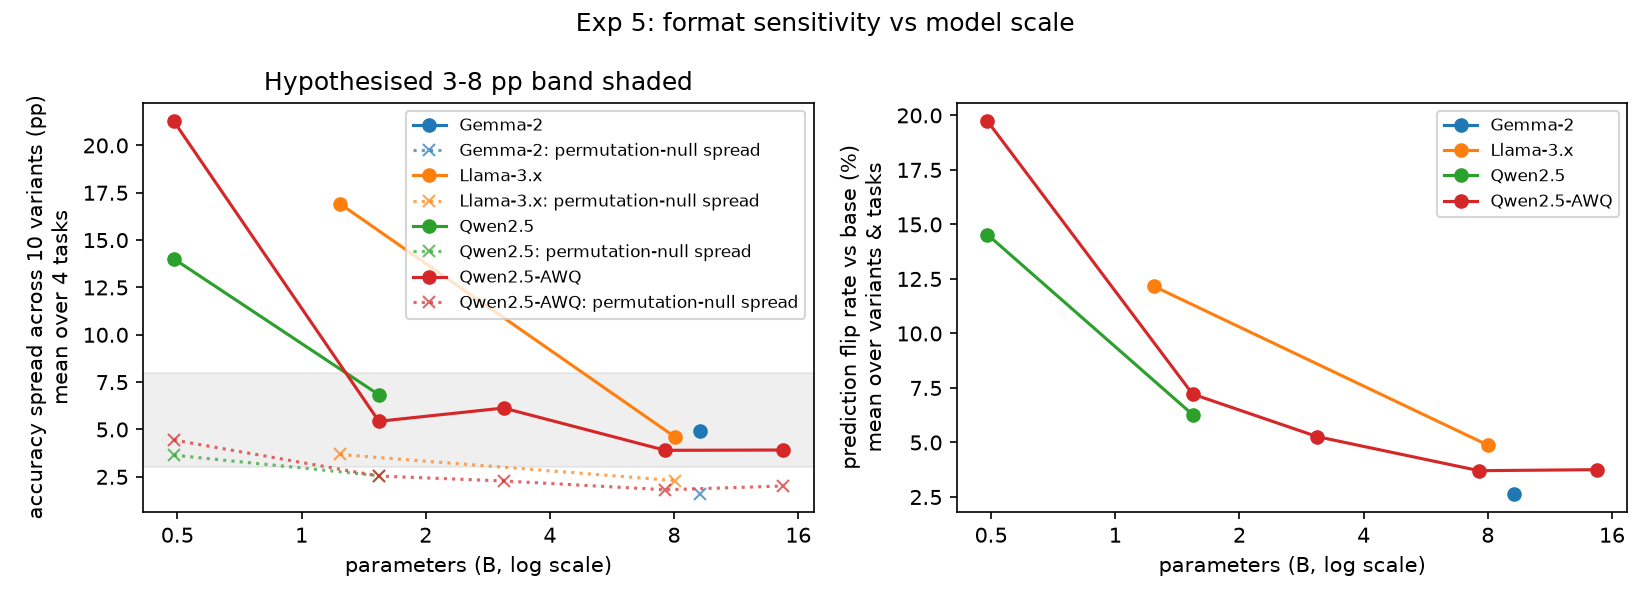
\includegraphics[width=0.95\linewidth]{figures/scale_sensitivity.png}
    \caption{Format sensitivity versus parameter count (log scale). \figleft Mean classification spread over four tasks; dotted lines with crosses show the permutation-null spread, and the shaded band is the hypothesized 3--8 pp range. \figright Mean prediction flip rate relative to \edit{base}. Sensitivity drops steeply from 0.5B to 1.5B and then flattens. qwen7b-awq and qwen14b-awq have the same mean spread (3.9 pp) and nearly the same flip rate (3.7\% vs.\ 3.8\%).}
    \label{fig:scale}
\end{figure}

\begin{table}[t]
    \centering
    \small
    \caption{OLS slope of per-model sensitivity on $\log_{10}(\text{params})$, i.e., change per tenfold increase in parameters. Negative slopes for spread and flip rate, and positive slopes for (negative) compliance and F1 deltas, mean less sensitivity at larger scale.}
    \label{tab:scale}
    \begin{tabular}{@{}llrrr@{}}
        \toprule
        \textbf{Metric} & \textbf{Models ($n$)} & \textbf{Slope / 10$\times$} & $p$ & \textbf{Spearman $\rho$} \\
        \midrule
        Classification spread & all (10) & $-$9.5 pp & \textbf{0.004} & $-$0.87 \\
        Classification spread & \qwen-AWQ ladder (5) & $-$10.6 pp & 0.084 & $-$0.80 \\
        Prediction flip rate & all (10) & $-$9.2 pp & \textbf{0.001} & $-$0.93 \\
        Prediction flip rate & \qwen-AWQ ladder (5) & $-$10.2 pp & 0.051 & $-$0.90 \\
        Mean $|\Delta|$ accuracy & all (10) & $-$2.2 pp & \textbf{0.012} & $-$0.84 \\
        ALL-CAPS compliance $\Delta$ & with \ifeval (9) & $+$1.6 pp & \textbf{0.028} & $+$0.79 \\
        Trailing-ws $|\log|$ length ratio & \qwen (7) & $-$2.1\% & 0.061 & $-$0.80 \\
        JSON-input F1 $\Delta$ & all (10) & $+$4.1 pp & 0.083 & $+$0.60 \\
        \bottomrule
    \end{tabular}
\end{table}

\Figref{fig:scale} and \tabref{tab:scale} relate sensitivity to model size. Across all ten models, spread falls by 9.5 points per tenfold increase in parameters ($p=0.004$, $\rho=-0.87$) and flip rate by 9.2 points ($p=0.001$, $\rho=-0.93$). However, the decline is concentrated below 1.5B. Along the \qwen-AWQ ladder, mean spread goes 21.3 $\to$ 5.4 $\to$ 6.1 $\to$ 3.9 $\to$ 3.9 points from 0.5B to 14B, and flip rate goes 19.7 $\to$ 7.2 $\to$ 5.3 $\to$ 3.7 $\to$ 3.8\%. A straight line in $\log(\text{params})$ fits this steep drop followed by a floor poorly. Part of the floor is item-level noise (null spreads of 0.7--3.1 points at 7--14B). Part of the decrease may also reflect higher base accuracy (52--63\% at the smallest sizes vs.\ 75--81\% at the largest), which leaves fewer items that can flip.

\para{Verdict on H5: directionally supported, but not log-linear.} Larger models are less format-sensitive, but the curve flattens at about 4 points of spread and 4\% flips from 7B to 14B.

%---------------------------------------------------------------
\subsection{Noise Floor and Idiosyncrasy of Edit Effects}
\label{sec:res_noise}

\begin{table}[t]
    \centering
    \small
    \caption{Noise floor of the inference stack. Placebo edits are byte-identical to \edit{base} after chat templating. Short classification outputs are almost unaffected by run-to-run nondeterminism, but long \ifeval generations often diverge, which moves compliance by up to $\sim$3 pp.}
    \label{tab:noise}
    \resizebox{\textwidth}{!}{%
    \begin{tabular}{@{}llcl@{}}
        \toprule
        \textbf{Check} & \textbf{Task} & \textbf{Identical outputs} & \textbf{Outcome difference} \\
        \midrule
        qwen1.5b-awq replicate run & classification & 99.7\% & max cell $|\Delta \text{acc}|$ 0.4 pp; edit-effect correlation $r=0.996$ \\
        qwen1.5b-awq replicate run & \ifeval & 76\% & length ratio 0.985; strict acc.\ $-0.7$ pp \\
        llama1b placebo & classification / \ifeval & 99.6\% / 23--31\% & max $|\Delta \text{acc}|$ 0.4 pp / length 0.98--0.99, strict $+1.5$ to $+2.8$ pp \\
        llama8b-awq placebo & classification / \ifeval & 99.8--99.9\% / 75--76\% & max $|\Delta \text{acc}|$ 0.4 pp / length 0.99--1.00, strict $-0.6$ to $-1.1$ pp \\
        gemma9b-awq placebo & classification & 99.7\% & 0.0 pp \\
        \bottomrule
    \end{tabular}
    }
\end{table}

\para{How noisy is greedy decoding?} \Tabref{tab:noise} shows that greedy decoding in \vllm is not bitwise deterministic across batch compositions. For classification, 99.6--99.9\% of outputs are identical across runs, and no cell moves by more than 0.4 points, which is far below the effects in \tabref{tab:spread}. For long \ifeval generations, only 23--76\% of outputs are identical. This alone moves strict compliance by up to 2.8 points (llama1b placebo), so \ifeval effects of about 3 points or less cannot be separated from inference noise. Separately, item sampling at $n=300$--$500$ produces a spread of 0.7--5.4 points (mean 2.7) even with no format effect, as the permutation nulls show.

\para{Do edit effects transfer across models?} Mostly not. Excluding \capsedit, per-cell edit effects correlate only weakly between the bf16 and 4-bit AWQ versions of the \emph{same} model ($r=0.28$ at 0.5B, $r=0.19$ at 1.5B), compared with $r=0.996$ between two runs of one model. Across other model pairs, correlations range from $-0.90$ (gemma9b-awq vs.\ qwen1.5b) to $+0.77$ (llama8b-awq vs.\ gemma9b-awq), with no clear family structure. Because effects at $\geq$7B are small, these correlations are noisy. Still, apart from the ALL-CAPS penalty, \emph{which} formats help or hurt behaves like model-specific noise, and even quantizing the same weights reshuffles it. Quantization also changes the \emph{magnitude} of sensitivity at small scale: 4-bit AWQ raises the mean spread of the 0.5B model from 14.0 to 21.3 points, while at 1.5B the two are similar (6.8 vs.\ 5.4).
